\section{Event-driven approach}
	In this chapter we aim at developping and implementing an algorithm for the simulation of a system driven by the mean-filed equation described before, and for a large number of nodes, in reasonnable times. The mean-field equation makes sense for an infinite number of actors and the actual number of neurons in most living beings is tremendous anyway (1e5 in drosophilia and 86 billions in human beings for instance).\\
	The usual way of carrying such a numerical simulation is to compute the finite difference integration of the associated diferential equation. There are several well-known methods based on this discrete-time approach, such that Euler or Runge-Kutta, but they all suffer from the same drawbacks: namely, the computational cost which is of order $N^2$, meaning the number of operations necessary on order to finish the simulation is of order the square of the number of neurons.\\
	Indeed, assuming there is on average $Nc\nu$ spikes per second (N the number of neurons, c the probability of connection between two neurons, $\nu$ the spike rate = on average a neuron emits $\nu$ spikes per second), and $\delta t$ is the time step, then there is on average $\frac{cN}{\delta t}$ updates per second (at each time step, only the spiking neurons and the post-synaptic ones are updated), but the average time elapsing between two spikes is $\frac{1}{Nc\nu}$. In order not to introduce errors due to the dynamical effect of a single spike, the time step should be so that the probability of receiving more than one spike in $\delta t$ is negligible. Put it otherwise, $\delta t<<\frac{1}{Nc\nu}$, and so $\text{average number of updates per second per neuron}>>N^2c^2\nu$, hence a complexity of order $N^2 per neuron$.\\
	In order to exceed this limit, we considered a different approach. Indeed, in realistic conditions the neurons emit at low rates but with a high variability in the time intervals between successive spikes, therefore a discrete-time algorithm will spend most of its time updating the state of the neurons, while the evolution of the potential of the membrane follows a deterministic law between two successive spikes. If the dynamic of a system is driven by these spikes (or more generally any instantaneous abstract event), then a more efficient algorithm can take advantage of the determinism of the state of a neuron between two spikes to interpolate its potential whenever a spike occurs, and only update the system when a new spike is emitted.\\
	Such an approach is called event-driven, and this is what is discussed hereafter. The complexity of this kind of algorithm is often linear in N, as a neuron influences an average of $Nc\nu$ other neurons per seconds, to be compared with the $N^2c^2\nu$ obtained before because of the very small time step necessary for not introducing a divergence too important. The simulation is also an exact solution of the equations driving the system, in that there is no approximation in the time of an event (except for the necessary rounding due to the limitation of real number representation on computers). This kind of algorithm is very effective, but much more complex to implement because of the event handling part.\\
	Altough this approach seems promising, it is not always appliable as so. One of the necessary conditions if the existence of a deterministic path from one state to another, and in the case of systems described by stochastic equations, this hypothesis may not be fulfilled. 
	This model is interesting because it seems to fit quite well to the assumptions necessary for event-driven simulations: the dynamic of the system is spike-driven and there is a quite deterministic evolution of the system between two spikes. On the other hand, there is a gaussian term that restrain the equation to the purely stochastic domain, as its values range in $\overline{\mathscr{R}}^+$, so the event-driven algorithm needs to be adapted to our specific needs. Thanksfully, the probability to generate a random number greater in absolute value, than an arbitrary bound decreases the higher the bound. In other words, if $X\sim\mathbb(\mu,\sigma^2), \mathscr{P}(\mu-r\sigma^2\leq X\leq\mu+r\sigma^2)=2\Phi(r)-1$, where $\Phi:\begin{cases}\mathscr{R}\to\mathbb{R}^+\\x\to\Phi(x)=\frac{1}{\sqrt{2\pi}}\int_{-\infty}^x e^{-\frac{t^2}{2}}dt\end{cases}$ is the cumulative distribution function of the gaussian distribution. Here r can be viewed as a confidence indicator, and so we can define a bound that will be almost surely an upper bound of the white noise.\\
	The first question that arise from this remark is how good is this confidence interval? With an infinitely large value of r the confidence is nearly 100\%, but then the upper-bound of the white noise is very large. On the table~\ref{tab:repartitionFunction} the actual values of the probability to generate out-of-boundary values are displayed. Even small values of r give a high enough confidence for several simulations, depending on the parameters chosen for the simulation, particularly the number of neurons. This brings back the discussion about the complexity of the algorithm: \todo{Add exact complexity}
	\begin{table}
		\centering
		\begin{tabular}{l||cccccc}
			\textbf{r}		& 1				& 2				& 3				& 4				& 5				& 6\\\hline
			$2-2\Phi(r)$	& 3.173105e-01	& 4.550026e-02	& 2.699796e-03	& 6.334248e-05	& 5.733031e-07	& 1.973175e-09
		\end{tabular}
		\caption{$P(r\leq\text{X OR X}\leq-r)=2-2\phi(r)$ (computed with R using \emph{pnorm} for a centered normalised law)}
		\label{tab:repartitionFunction}
	\end{table}

\section{Rejection sampling method}
	As a reminder, here is the model of the system as presented in the previous chapters:
	\begin{equation*}
		\text{Equation of the model}
	\end{equation*}\todo{Put the equation of the model}
	This kind of stochastic equation is often solved using a rejection sampling method. This method is used for generating random numbers from a target distribution X with the probability distribution function f(x), using another distribution Y of probability distribution function g(x). The idea is that generating numbers from the proposed distribution Y shall be easier than generating numbers directly from X, so that one can generate a large set of numbers from Y and then sample them, accepting with a probability $\frac{f(x)}{g(x)}$. There is a condition of course that f and g must satisfy $f(x)\leq g(x)$ for all x. Also, even if that is not necessary, there is another condition that $f(x)\approx g(x)$, otherwise the rejection sampling method rejects too many propositions. The figure~\ref{fig:rejectionSampling} exposes this process, with a non usual pdf f and a very classical piecewise constant pdf g.
	\begin{figure}
		\begin{center}
				\begin{tikzpicture}[scale=2]
					\draw [-latex] (-0.1,0) -- (5.1,0) node[right] {x};	% X-absciss
					\draw [-latex] (0,-0.1) -- (0,2.5) node[left] {y};	% Y-absciss
					
					\draw (0,1) -- (1,1);
					\draw [domain=0:1] plot (\x,{(\x-1)*(\x-1)});
					\draw [fill] (0.1,0.9) circle (0.01);
					\draw [fill,red] (0.1,0.1) circle (0.01);
					\draw [fill] (0.5,0.45) circle (0.01);
					\draw [fill] (0.8,0.7) circle (0.01);

					\draw [dashed] (1,1) -- (1,2);
					\draw (1,2) -- (2,2);
					\draw [domain=0:1] plot (\x+1,{sin((2*pi*\x-pi/2) r)+1});
					\draw [fill] (1.1,1.5) circle (0.01);
					\draw [fill,red] (1.5,1.5) circle (0.01);
					\draw [fill] (1.8,1.9) circle (0.01);
					\draw [fill,red] (1.8,0.2) circle (0.01);

					\draw [dashed] (2,2) -- (2,1.5);
					\draw (2,1.5) -- (5,1.5) node [above] {y=g(x)};
					\draw [domain=0.001:60,samples=200] plot (\x/20+2,{1.5*exp(-4/(\x))}) node [below] {y=f(x)};
					\draw [fill] (2.1,1) circle (0.01);
					\draw [fill,red] (3.5,1) circle (0.01);
					\draw [fill] (4.8,1.45) circle (0.01);
					\draw [fill,red] (4.8,0.45) circle (0.01);
					% \foreach \x in {0,...,5}{
					% 	\tikzmath{\x = 3 * rnd + 2;
					% 				\y = 1.5 * rnd;
					% 				\yy = 1.5 * exp(-4 / \x);}
					% 	{\draw [fill,"\ifthenelse{\y<\yy \OR \y=\yy}{color=red}{color=black}"] (\x,\y) circle (0.01);}
					% };
				\end{tikzpicture}
			\end{center}
			\caption{Illustration of the rejection sampling method. g(x) is the PDF of the proposed distribution Y and f(x) is the PDF of the target distribution X. The points are first generated following the Y distribution, then sampled and accepted only if they follow the X distribution, i.e. their value is less than the one of the pdf f. There are five accepted points (in red) and seven rejected points.}
			\label{fig:rejectionSampling}
	\end{figure}
	As can be seen on the figure~\ref{fig:rejectionSampling} the acceptation rate is often quite low because it can be hard to find a pdf g matching the target pdf f. Also the approximation pdf must at any time have higher values than the target pdf, meaning sometimes it does not even exist.


\section{Definitions}
	With this approach some definitions given before are no longer appliable to the system.\\
	The threshold is then defined as:\\
	At any given time, any neuron i of potential $V_i$ has a chance of firing which is function of
	\begin{equation*}
		f(V_i)=S*(Pos(V_i-V_T))^E\text{, where }Pos(x)=\begin{cases}x & \text{if }x>0\\V_R & else\end{cases}
	\end{equation*}
	$V_T$ is chosen equal to one, and $V_R$ is equal to zero for all neurons (for simplicity purposes), but they could be chosen more randomly. A threshold value too low (too close to the reset value) is problematic, as it means that potentials are going to reach their threshold quickly after a neuron has spiked (in which case the system is "stuck" in a perpetual series of spikes). By design only one neuron can fire at a given time (the spike trains are point processes), and if a cascade is cannot normally happen (except in cases where some values are rounded to zero due to the limitations in floating point precision, but more on that later) that does not solve the issue of blow-up, as a similar phenomenon can still occur (the rate will not tend to infinity, still it tends to very high values). The blow-up is indeed newly defined as (Pertinence de comparer \`a N lorsque tous les neurones ne spikent pas ? Pourquoi pas plut\^ot quelque chose du type $1/\delta_N->\infty$, avec $\delta_N$ l'intervalle entre deux spikes ?):
	\begin{equation*}
		\frac{1}{\delta_N}>Constant\text{, typically N}
	\end{equation*}
	where $\delta_N$ is an interval between two spikes (or a mean interval, or a moving average). The constants S and E are chosen so that the chances of fire are high even for values of the potential low above the threshold (typically, $S=10^5\text{ and }E=5$, while values of potentials at spiking times are around [CALCULER VALEUR PRECISE, DE MEMOIRE 1.4]).

	The system is driven by a stochastic PDE and discontinuities are randomly introduced depending on the value of parts of the system. There are two common ways of simulating a stochastic PDE. The Euler-Maruyama method for numerical approximation of stochastic differential equations results in the construction of a Markov chain on the interval $[0,T]$ of simulation. While quite simple to set up and understand, it is wastefull for processes that spend a lot of time not changing, in this case not spiking. In addition, the resolution of the time interval shall be low enough to capture the meaningful variations in the system, here the moments of spikes and the blowing-up behaviour, as well as to keep the simulation precise enough. Spikes are diracs, discontinuities of the system, and the blow up happens when the firing rate tends to infinity, or to spell it otherwise, when the time interval between spikes tends to zero.\\
	The second method is the rejection sampling, which is a common method for generating random numbers from distribution of not well defined cumulative distribution function \url{http://www.aip.de/groups/soe/local/numres/bookcpdf/c7-3.pdf}. Here the stochastic process is the network of neurons, and its intensity directly depends on the potentials of the neurons, following the function $f:\mathbb{R}\rightarrow\mathbb{R}^+$ described above. In this method two numbers (for the one dimension case) are generated, $(t,u)\in\mathbb{R}+\times[0,1]$. They represent a point in the plane and depending on whether the point can be placed under the curve of the desired cumulative distribution function or not the point will be declared accepted or rejected. In order to achieve this in practice the value of $\frac{f(x)}{f_{max}(x)}$ is compared to a number uniformly generated between zero and one. The approximation function is used in order to increase the probability of generating a point under the curve (on the full spectrum of real positive numbers, the chances are null).\\

	
	\todo{INCLUDE A GRAPHIC EXAMPLE OF THE PROCEDURE, ALIKE THE ONE DRAWN ON BOARD}

	The $f_{max}$ here can be computed by a simplified, limit in time version of the model. Indeed, a rough estimate can be created by dividing the equations in sums of which the maximum value in time will be taken.
	\[
		f_{max}=\max_t(a+\exp^{-\lambda t}(y_t^i-y_S^i))+\max_t(\sigma\mathbb{N}(0,\frac{1-\exp^{-2\lambda t}}{2\lambda}))
	\]
	The maximum proposed here is not correct. Indeed, there are no boundaries for a normally distributed random number, hence the white noise cannot be bounded and the variations for the potentials are in $\mathbb{R}\cup\{-\infty,\infty\}$... But! The chance of generating a number of absolute value larger than the variance decreases the farther away this number is from the variance. Thus it is possible to consider, with a certain degree of confidence, that no numbers will be generated outside of a predefined interval, the bounds of which will constitute our maximum. More precisely, given a random variable X following a normal law $X~\mathbb{N}(\mu,\sigma^2)$, then it is possible to compute $P(\mu+k\sigma\leq X)$. The table \hyperref[repartitionFunction]{\ref{tab:repartitionFunction}} gives values of the chances of generating a number outside the interval $[\mu-k\sigma,\mu+k\sigma]$.\\
	In the current implementation k has been fixed at 5, as the number of neurons will hardly be higher than $10^5$ for memory reasons (the graph of interaction takes $p\times N^2\times 64$ bits of ram memory, p being the probability of connection between two neurons in a Erdos-Renyi graph, 64 being the number of bits necessary for representing an integer on a typical computer nowadays and for $N=10^5$ this value is higher than the typical amount of ram available on a computer, even for dedicated comptuting machines). There is also an influence of the number of spikes (accepted or rejected) generated during the simulation: each time the simulator decides whether the spike is accepted or not the true value of the potential is computed therefore the value of the noise is computed and there is a chance of generating a normally distributed number higher than the bound we have set.\\

	So tosummarize, we have chosen to use a thinning procedure to compute the solution of the stochastic partial differential equation described in the \ref{sec:Model}. The thinning procedure necessitates the use of an approximation function, which must be in any point higher than the function to simulate/compute. Even though a part of our model is a gaussian white noise, which is unbounded, it is still possible to use a pseudo-boundary for the noise, that is to say a number that will constitute an upper-limit with a certain degree of confidence. The limit directly depends on the confidence interval we want for our simulation, so this solution is both easy and flexible. Computing this pseudo-boundary necessitates only values that are necessary to compute the value of the gaussian white noise, so this solution does not increase the amount of computations needed. Actually it is much less expensive, in processor time, to compute the value of the upper-limit, as the actual value of the variance (which relies on an exponential in our case) is not needed (a maximum in time of the variance is enough, and adds in the confidence). Also, it is important to remark that even if we have focused on giving an upper-bound to the noise, there are other parts in our model that are approximated too, and so values of the noise not too much above the upper-limit may not make our approximation function $f_{max}$ lesser than the actual potential, so the solution is robust even to small errors.\\

	Finally, we can remark that we are sampling the noise anyway, meaning there is no way for us to know that even if the noise at the time of spike is indeed in the boundaries, it has not crossed the boundaries during the time inbetween two consecutive spikes. So what if there are errors in the evaluation of the noise? Two cases emerge. First, there is a bad approximation of the noise of the spiking neuron. So this neuron is certainly the good one to pick for a spike but it may have spiked a bit earlier if we had the information of the real value of its potential. The second case is more criticial, as this is the case where a neuron has been chosen for spiking, but the potential of one of the non chosen neurons is higher than expected, meaning it had actually more chance to spike. Of course the neuron we have chosen may actually still be the good one, then the error does not matter at all, the next computation of the potential shall rectify the mistake. Yet, even if we imagine that having another estimation for the potential would have changed the spiking neuron, given that we are dealing we at minimum 10,000 neurons, and more probably 100,000 neurons, and generating around the same number of spikes, having even a handfull of mistakes would not mean a large deviation of the final result (if a neuron should have spiked but does not, and this because of the noise, not the configuration of the network or the intensity of the spikes or whatever, then it will spike just a bit later, and excepting in the case where we speak about very critical neurons of very specific networks, this kind of mistakes can be considered as a good tradeof for speed).\\

	At this stage we have a first draft for the thinning procedure algorithm, but we can improve it a lot. For now we have focused on improving the efficiency of and discussing about the quality of the approximation function $f_{max}$, but f is not the real equation simulated here, it just helps defining a probability for a neuron to spike, depending on the value of its potential. But as the potential evolves in time, the approximation is always false, and by a bigger margin at the beginning of time than at infinity, since the approximation function is built using the values for $t\rightarrow\infty$. Unfortunately, the values of t (the x-axis part of the points generated for the thinning method) have a lot more chance to be small as they are generated using an exponential distribution (we are dealing with poisson processes so the spikes must be exponentially distributed in time [enfin ici du moins en l'occurrence c'est en temps]). This is also an issue for the random generation, as pseudo-random number generators cycle and generating more unuseful numbers may lead the generator to cycle.\\

	A common solution to avoid this is to bound the research of accepted points in time: we define a time interval of research and then look for points in this interval. Once a certain condition is met (for instance here every time we have an accepted point or when the time for the next potential spike is greater than the time limit) we stop or change the time interval. This way the approximation function is way closer to the real function and we can drastically improve the amount of accepted points.\\

	\todo{INSERT HERE GRAH OF THINNING METHOD WITH TIME INTERVALS}

\section{Algorithm in pseudo code}
	Finally here is, in pseudo code, the algorithm used for simulating the equation driving our model.\\

	\begin{algorithm}
		\caption{Pseudo code of the thinning algorithm used for simulating the system}
		\label{alg:pseudo-code}
		\begin{algorithmic}
			\State Initialize all parameters
			\Repeat
				\Repeat
					\State determine an interval $[t_{n-1},t_n]$ on which sampling
					\State compute the array of $f_{max}(Y_{t_{n-1}})$ and $\sum f_{max}(Y_{t_{n-1}})$ on interval $[t_{n-1},t_n]$
					\State $t_n\sim t_{n-1}+\mathscr{E}(\sum f_{max})$
				\Until{not in good interval or all $f_{max}$ are at 0}
				$u\sim\mathbb{U}([0,1])\rightarrow \mathbb{P}(\text{spiking neuron is neuron i})=\frac{f_{max}^i(Y_{t_n}^i)}{\sum_j^N f_{max}^j(Y_{t_n}^j)}$
				$u\sim\mathbb{U}([0,1])\rightarrow \mathbb{P}(\text{accepting spike of neuron i})=\frac{f^i(Y_{t_n}^i)}{f_{max}^i(Y_{t_n}^i)}$
				\If{ spike is accepted }
					update the potentials of all postsynaptic neurons
				\EndIf
			\Until{do not have the good amount of accepted spikes}
		\end{algorithmic}
	\end{algorithm}

\section{Improving efficiency}
	\todo{PENSER A METTRE UN PEACH SUR OPENMP, LES ALTERNATIVES ET PK ON (JE) L'A CHOISIS}
	This section will mainly focus on speed and memory usage. The algorithm presented above works perfectly except that the computations involved here can be very long in processor time, and that the amount of memory for running it is potentially tremendous. On the speed part, the algorithm has been implemented in C and optimised using -O3 in order to take advantage of the gain of speed of the low level languages. Dedicated libraries (here openmp) can and have been used in order to improve the speed of some parts of the simulation, in the parts where a state variable needs to be changed for all or a large amount of neurons.
	Some specific interaction cases, like full connection (including selfconnections), complete interaction graph and independence (no connections) are encoded so that the connection graph is not needed, improving speed and memory consumption. but on the generic case, even though the full matrix of interactions is not stored (only the relevant parts), the memory for storing the interaction graph takes around $p*N^2$, where p is the probability of interaction and N the number of neurons. For even $10^5$ neurons that makes about 1 GB, given 1 byte is enough to store the index of neurons (and the addresses in memory)(spoiler: it is not, and takes rather 4 times more) and with a probability of connction of 0.1... where the probability of connection was 1 in the mathematical papers.\\

	Still, when the interaction graph is too big but there is no way to skip the generation of the interaction graph, there is a way to save a lot of memory by storing seeds instead of a boolean about whether there is an interaction or not. When generating an interaction graph with a random connection probability, for each neuron, instead of storing an array containing alll the postsynaptic neurons, one can rather store the state of the random number generator (for instance, in Mersenne Twister, it is about 128 bits, and it is one of the largest state for a classical random number generator) just before randomly chosing the postsynaptic neurons. This way, each time a neuron is spiking, one can regenerate the same graph, and more interestingly the specific part of the interaction graph of interest (that is to say only the postsynaptic neurons of the spiking neurons, and no the entire graph of interaction). While a lot slower, this method is probably one of the most efficient in memory, taking advantage of the pseudo character of the random number generation in computer science.\\

	This method is also parallizable with openmp or any library alike it, but it is more difficult to achieve if one want to guarrantee the reproducibility of the results. The parallelization is possible because if one cuts the array of the postsynaptic interactions in k parts, then k random number generators can be used for generating the interaction graph. The issue here is on the initialization of the random number generators, as we want to avoid the case where there is an overlapping in the sequences in use by two threads at the same time. A RNG like the Mersenne Twister, with a very large pseudo period is great for this purpose, as it allows to cut the pseudo period so that two processes correctly seeded will never overlap. This considerations are also needed if one wants to run several simulations in parallel. [METTRE PUBLI BENNIE]

\section{Implementation}
	As said before, the algorithm was finally implemented in C (and prototyped in Java). There are several reasons for that. The C language is close enough to the machine language to be one of the fastest possible and allows a precise management of the memory usage. Most compiler (as gcc, the one we used) also have options for improving the speed and memory consumption of the program. These options are also supported by the version of the Mersenne-Twister random number generator used in the implementation. There are two of them, on for integer generation and one for double precision generation, and they can be found at \url{http://www.math.sci.hiroshima-u.ac.jp/~m-mat/MT/SFMT/index.html}. O this site there are more information about Mersenne-Twister generators in general, as this page has been created and is maintained by one of their creator, Makoto Matsumoto.\\

	The computations at stake here involve potentially both very low and very high values. For instance the time of spikes are exponentially distributed. They are obtained using an exponential distribution of parameter the sum of all the approximation functions (on the current interval of work). This value can typically raise up to $10^5$ or $10^6$ (consider the same number of neurons, their potential close to the threshold).\\

	For this reason some 

\section{A word about the rng}
	Mersenne twister, and not xorshift because the mersenne allows for a reproduction of the simulations, which is also necessary for a part of the algorithm. It is well known, and has a huge period which is important for a part of the algorithm. Also there are a lot of good implementations, some of the creator itself who actively update them when bugs or improvements are found. The method also allow for good generation of random real numbers (not only integers)

	A related subject is the distribution followed by the random numbers. The algorithm presented earlier needs several random numbers from various distributions, none of them being too exotic (uniform numbers with arbitrary upperbound and normal numbers centered on zero with arbitrary variance), but as the library used only provide uniform random series of 32 or 64 bits and random floating point numbers in [1,2) or {[0,1], [0,1), (0,1], (0,1)}, we must implement a way to generate the numbers drawn from our arbitrary distributions. In both cases a sampling method (again) is used, and we are going to describe them.

	First the uniform case. We have a random integer generator, and we assume it gives perfectly random numbers in $ {0, 1, ..., M} $, while we want uniform numbers in $ {0, 1, ..., U} $. A common method to achieve this is to use a modulo: $ \mathbb{U}([0, M]) mod[U+1] $. The issue here is that unless M is a multiple of $ U+1 $, the uniformity of the numbers is lost using this method. The case in which the method works can be used as a trick for guarrantying uniformity though. Indeed, if M is not a multiple of $ U+1 $, there must exist one that is lower than M but close anyway. Knowing that, we can simply take any number that is lower than $ U+1 $ and in the rare cases a number greater than $ U+1 $ is drawn, we just have to reject it and draw another one. Of course the maximum value M must be quite high, compared to $ U+1 $ in order for this method to be effective. For instance, if $ U+1= $, there is a 49\% of rejection. If the rest of the euclidean division of M bu $ U+1 $ is U, the 

	\begin{figure}
	\begin{center}
		\begin{tikzpicture}[samples=200,scale=2,
							dot/.style={circle,inner sep=1pt,fill,label=180:$#1$,name=#1}]
			\coordinate (O) at (0,0);
			\tikzmath{
						\tmax=7;		\conf=.5;	\xplotmax=.75;	\xmax=\xplotmax+\conf+.5;
						\thresh=.5;
						\t1=2;	\t2=4;	\t3=5;	\taccepted=6.5;
						\y1=\xplotmax*(1-exp(-\t1));	\y2=\xplotmax*(1-exp(-\t2));	\y3=\xplotmax*(1-exp(-\t3));	\yaccepted=\xplotmax*(1-exp(-\taccepted));
			}
			\coordinate (T) at ($(O)+(\tmax,0)$);
			\coordinate (Poisson) at ($(O)+(1,-1)$);

			\draw [name path=x-absciss, -latex] ($(O)+(-0.1,0)$) -- ($(O)+(\tmax,0)$) node [right] {t};
			\draw [name path=y-absciss, -latex] ($(O)+(0,-0.1)$) -- ($(O)+(0,\xmax)$) node [left] {X(t)};

			\draw [name path=threshold, dashed] ($(O)+(0,\thresh)$) node [left] {$V_T$} -- ($(O)+(\tmax,\thresh)$);

			\draw [name path=plot 1, domain=0:\taccepted,thick] plot (\x,{\xplotmax*(1-exp(-\x))});
			\draw [dotted, name path=plot 2, domain=0:\taccepted] plot (\x,{\xplotmax*(1-exp(-\x))+\conf});

			\path [name intersections={of=threshold and plot 2,by=E}];

			\coordinate (E2) at ($(O)!(E)!(T)$);
			% \draw [thick,decoration={brace,mirror,raise=0.5cm},decorate] (O) -- (E2) node [pos=0.5,anchor=north,yshift=-0.55cm] {Jump};
			% \draw [thick,decoration={brace,mirror,raise=0.5cm},decorate] (E2) -- (T) node [pos=0.5,anchor=north,yshift=-0.55cm] {Rejection sampling};
			\path [name path=truc] (E) -- (E2);
			\path [name intersections={of=plot 1 and truc,by=E3}];
			% \node [fill=red,inner sep=1pt,label=-90:$E3$] at (E3) {};
			\draw [dashed] (E3) -- (E);

			\node at (0,-0.2) {Sampling};
			\draw [vecArrow] (\t1,-0.3) node [below] {rejected} -- (\t1,0);
			\draw [innerWhite] (\t1,-0.3) -- (\t1,0);
			\draw [vecArrow] (\t2,-0.3) node [below] {rejected} -- (\t2,0);
			\draw [innerWhite] (\t2,-0.3) -- (\t2,0);
			\draw [vecArrow] (\t3,-0.3) node [below] {rejected} -- (\t3,0);
			\draw [innerWhite] (\t3,-0.3) -- (\t3,0);
			\draw [vecArrow] (\taccepted,-0.3) node [below] {accepted} -- (\taccepted,0);
			\draw [innerWhite] (\taccepted,-0.3) -- (\taccepted,0);

			\draw [<->] (\t1,\xplotmax+.1) node [dot=A] {}-- (\t1,\y1) node [midway,right] {$W_t$};
			\draw [<->] (\t2,\xplotmax+.35) node [dot=B] {} -- (\t2,\y2) node [midway,right] {$W_t$};
			\draw [<->] (\t3,\xplotmax-.3) node [dot=C] {} -- (\t3,\y3) node [midway,right] {$W_t$};
			\draw [<->] (\taccepted,\xplotmax+\conf-.1) node [dot=D] {} -- (\taccepted,\yaccepted) node [midway,right] {$W_t$};

			\draw [name path=plot 3, domain=0:\tmax-\taccepted,thick] plot (\x+\taccepted,{\xplotmax*(1-exp(-\x))});
			\draw [dotted, name path=plot 4, domain=0:\tmax-\taccepted] plot (\x+\taccepted,{\xplotmax*(1-exp(-\x))+\conf});

			\draw ($(O)+(0,\xplotmax+\conf)$) node [left] {$X_{max}$} -- ($(O)+(\tmax,\xplotmax+\conf)$);
		\end{tikzpicture}
	\end{center}
	\caption{Rejection sampling procedure for a stochastic system with random noise $W_t$}
	\label{fig:rejectaccept}
\end{figure}
	\begin{figure}
	\begin{subfigure}{.45\textwidth}
		\centering\begin{tikzpicture}
			\tikzmath{
						\length=4;	\height=3;
			}
			\draw (0,0) rectangle (\length,\height) node [midway] {$\mathscr{M}_{i,j}=1$};
			\node [above] at (0,\height+.1) {1};
			\node [above] at (\length/2,\height+.1) {j};
			\node [above] at (\length,\height+.1) {n};
			\path (0,\height+.1) -- (\length/2,\height+.1) node [above,midway] {$\cdots$} -- (\length,\height+.1) node [above,midway] {$\cdots$};

			\node [left] at (-.1,\height-.1) {1};
			\node [left] at (-.1,\height/2) {i};
			\node [left] at (-.1,0) {n};
			\path (-.1,\height-.1) -- (-.1,\height/2) node [left,midway] {$\vdots$} -- (-.1,0) node [left,midway] {$\vdots$};
		\end{tikzpicture}
		\caption[Matrix of children]{Matrix of children $\mathscr{M}_{i,j}=1$ if j is children of i and 0 otherwise.}\label{fig:mat}
	\end{subfigure}
	\begin{subfigure}{.45\textwidth}
		\centering\begin{tikzpicture}[implies/.style={double,double equal sign distance,-implies}]
			\tikzmath{
						\length=1;	\height=3;
						%\length2=5-1.25;	\height2=1;
			}
			\draw (0,0) rectangle (\length,\height) node [midway] {$V^s$[i]};
			\node [above] at (\length/2,\height+.1) {1};
			\node [left] at (-.1,\height-.1) {1};
			\node [left] at (-.1,\height/2) {i};
			\node [left] at (-.1,0) {n};
			\path (-.1,\height-.1) -- (-.1,\height/2) node [left,midway] {$\vdots$} -- (-.1,0) node [left,midway] {$\vdots$};

			\draw (\length+.25,\height/2) edge[implies] (\length+1,\height/2);

			\node [above] at (\length+1.25,2.1) {1};
			\node [above] at (\length+1.25+3.75/2,2.1) {j};
			\node [above] at (\length+1.25+3.75,2.1) {n};
			\path (\length+1.25,2.1) -- (\length+1.25+3.75/2,2.1) node [above,midway] {$\cdots$} -- (\length+1.25+3.75,2.1) node [above,midway] {$\cdots$};
			\draw (\length+1.25,\height/2-.5) rectangle (\length+5,\height/2+.5) node [midway] {$V^c_i$[j]};
		\end{tikzpicture}
		\caption{Vector of seeds and reconstructed vector of children}\label{fig:vect}
	\end{subfigure}\\
	\centering\begin{subalgorithm}{\textwidth}
		\begin{algorithmic}[1]
			\State RNG: a random number generator
			\State p: probability of connection between two neurons
			\State $\mathscr{M}_{i,j}$: matrix of interaction
			\Function{Interaction matrix}{RNG, p}
				\ForAll{$(i,j)\in\{1,\cdots,n\}^2$}
					\State $\mathscr{M}_{i,j}\gets\Call{RNG.B}{p}$
				\EndFor
			\EndFunction
		\end{algorithmic}
		\caption{Generation of a matrix of children}\label{alg:mat}
	\end{subalgorithm}\\
	\centering\begin{subalgorithm}{\textwidth}
		\begin{algorithmic}[1]
			\State RNG: a random number generator
			\State p: probability of connection between two neurons
			\State $V^s$: vector of states
			\State $V^c_i$: vector of children of neuron i
			\Function{Reconstructible}{RNG, p}
				\For{i}{1}{n}
					\State $V^s_i\gets$\Call{RNG.State}{}
					\For{j}{1}{n}
						\State \Call{RNG.B}{p}\COMMENT{Generate, \textbf{without storing them}, the children of i}
					\EndFor
				\EndFor
				\RETURN $V^s_i$
			\EndFunction
			\Function{Reconstruct}{RNG, i, $V^s$}
				\State \Call{RNG.setState}{$V^s$[i]}
				\For{j}{1}{n}
					\State $V^c_i[j]\gets$\Call{RNG.B}{p}
				\EndFor
				\RETURN $V^c_i$
			\EndFunction
		\end{algorithmic}
		\caption{Generation of a vector of rng states}\label{alg:vect}
	\end{subalgorithm}
	\caption{Algorithm for generating erdos-reynii graph in memory (a and c) and reconstructible (b and d)}
	\label{fig:rec}
\end{figure}

	\begin{figure}
	\begin{center}
		\begin{tikzpicture}[scale=1]
			\coordinate (O) at (0,0);

			\tikzmath{
						\tmax=5;	\ymax=2;
						\x0=.1;	\x1=\tmax/2;	\x2=\tmax-.5;
			}

			\draw [-latex] ($(O)+(-0.1,0)$) -- ($(O)+(\tmax,0)$) node [right] {t};
			\draw [-latex] ($(O)+(0,-0.1)$) -- ($(O)+(0,\ymax)$) node [left] {X(t)};

			\draw [dotted] ($(O)+(0,\ymax-.5)$) node [left] {$V_T$} -- ($(O)+(\tmax,\ymax-.5)$);

			\draw [-latex] ($(O)+(\x0,-.2)$) node [below] {Beginning} -- ($(O)+(\x0,0)$);
			\foreach \k in {0,...,5}{
				\tikzmath{
							\x = \x0;
							\y = 0.25 * rnd;}
				\draw ($(O)+(\x,\y)$) node {$\cdot$};
			};

			\draw [-latex] ($(O)+(\x1,-.2)$) node [below] {During simulation} -- ($(O)+(\x1,0)$);
			\foreach \k in {0,...,5}{
				\tikzmath{
							\x = \x1;
							\y = 0.25 * rnd + 0.5;}
				\draw ($(O)+(\x,\y)$) node {$\cdot$};
			};

			\draw [-latex] ($(O)+(\x2,-.2)$) node [below] {Near first spike} -- ($(O)+(\x2,0)$);
			\foreach \k in {0,...,5}{
				\tikzmath{
							\x = \x2;
							\y = .25 * rnd + 1.35;}
				\draw ($(O)+(\x,\y)$) node {$\cdot$};
			};
		\end{tikzpicture}
		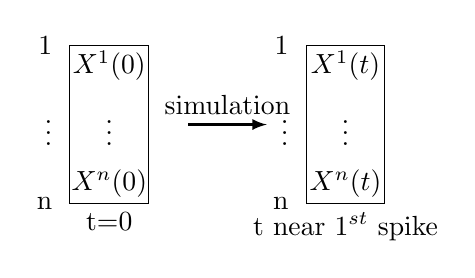
\begin{tikzpicture}[scale=1]
			\draw (0,0) rectangle (1,2);
			\node [left] at (-.1,2) {1};		\node at (.5,1.75) {$X^1(0)$};
			\node [left] at (-.1,1) {$\vdots$};	\node at (.5,1) {$\vdots$};
			\node [left] at (-.1,0) {n};		\node at (.5,.25) {$X^n(0)$};
			\node [below] at (.5,0) {t=0};
			
			\draw [thick,-latex] (1.5,1) -- (2.5,1) node [midway,above] {simulation};

			\draw (3,0) rectangle (4,2);
			\node [left] at (2.9,2) {1};		\node at (3.5,1.75) {$X^1(t)$};
			\node [left] at (2.9,1) {$\vdots$};	\node at (3.5,1) {$\vdots$};
			\node [left] at (2.9,0) {n};		\node at (3.5,.25) {$X^n(t)$};
			\node [below] at (3.5,0) {t near $1^{st}$ spike};
		\end{tikzpicture}
	\end{center}
	\caption{Illustration of the initialisation process, the state of the system is represented at different instants of the simulation (each dot is a neuron, x-absciss time and y-absciss the potential of the neuron).}
	\label{fig:init}
\end{figure}